
\begin{titlepage}
	\begin{center}

		\vspace{30mm}
		
		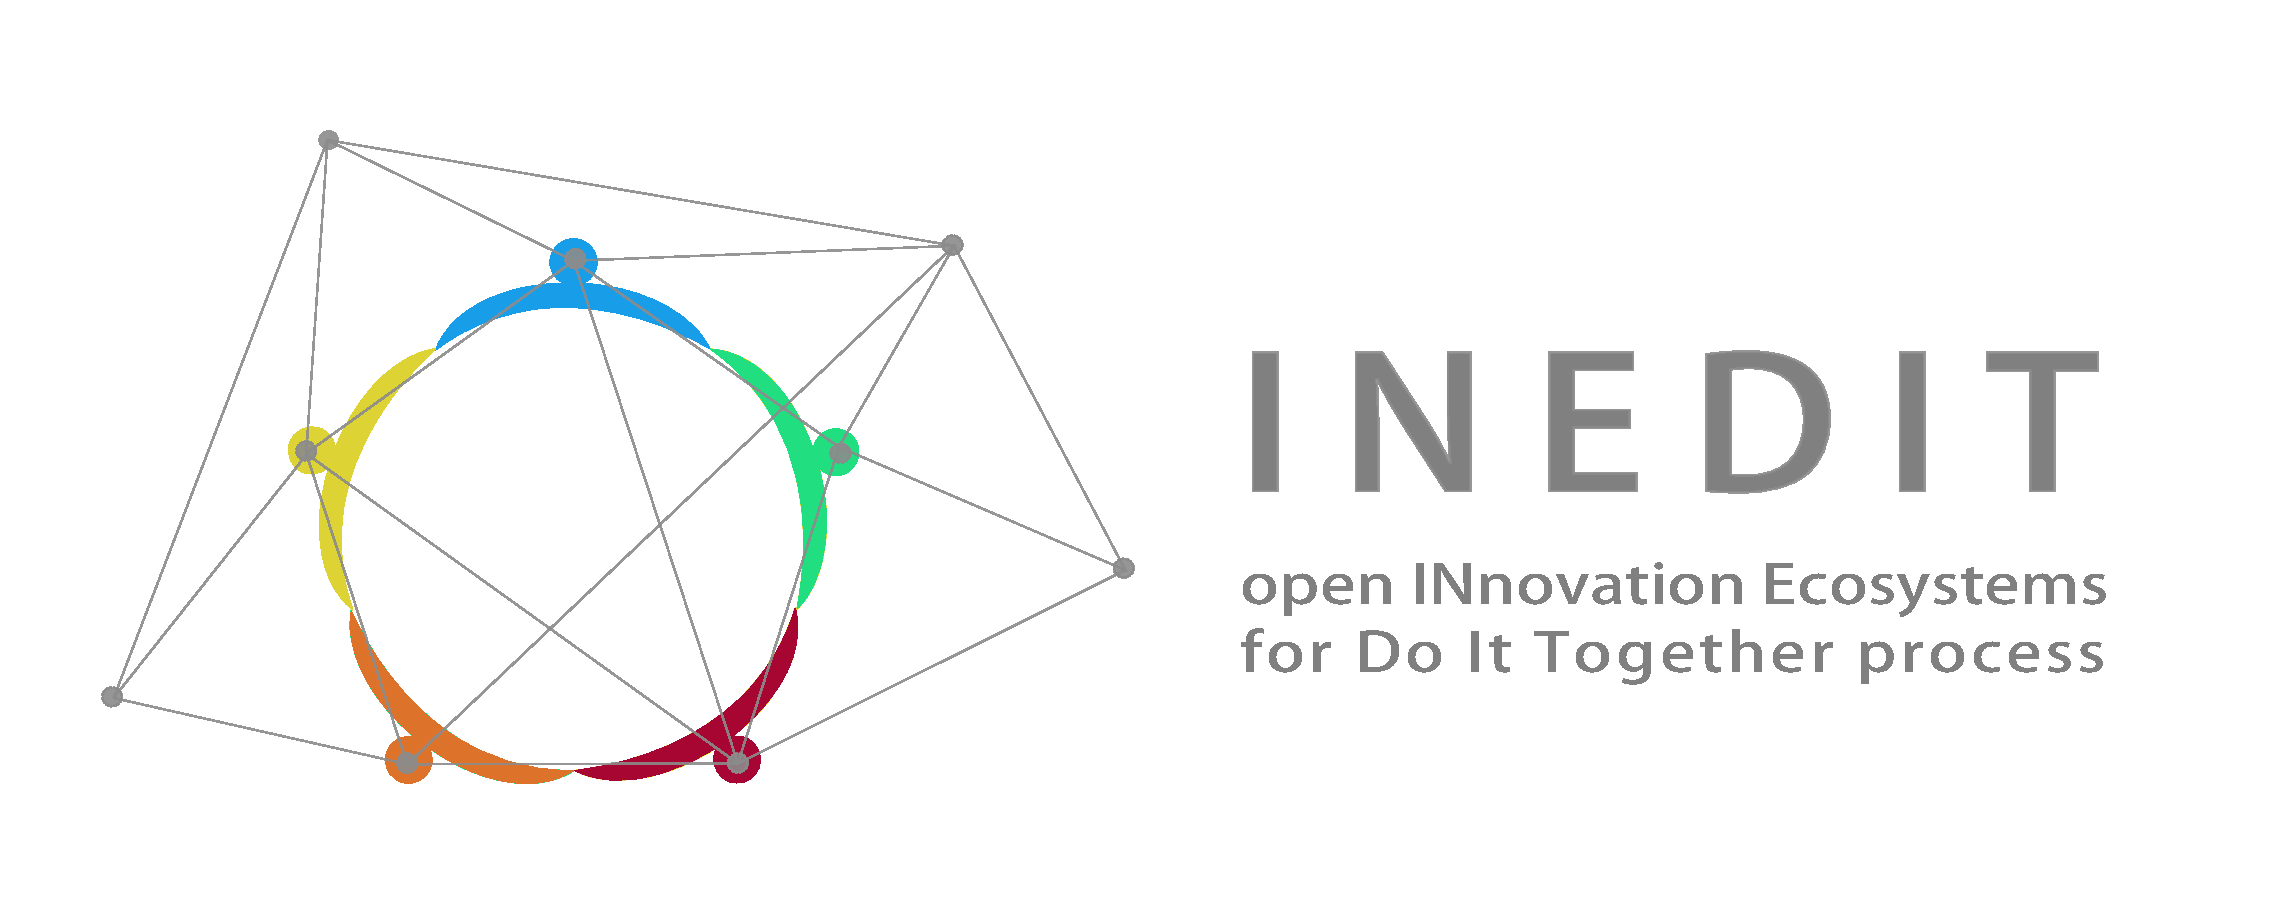
\includegraphics[width=\linewidth]{figures/Inedit_horiz.pdf}\\ 
		
		\vfill
		
		\textbf{\Huge{\textcolor{darkgray}{ D6.4 3D Printing of recycled plastic demonstrator }}} \\ 
		
		\vfill
		
		\vspace{60mm} 
		
		
		
      \textcolor{gray}{\rule{\textwidth}{2pt}}
      
		\vspace{5pt}
		\begin{tabular}{ c p{8cm} c }
           & & Version 3.0  \\ 
         WP6 T6.4  & & March 2023   \\ 
      \end{tabular}
		\vspace{5pt} 
		
		\textcolor{gray}{\rule{\textwidth}{2pt}}
		
		
	
		
		\vfill
		
	\end{center}
\end{titlepage}

\newpage



\begin{tabu} to \textwidth { X  X[0.7] | X | X }
\toprule


\multicolumn{2}{l |}{ \multirow{4}{*}{  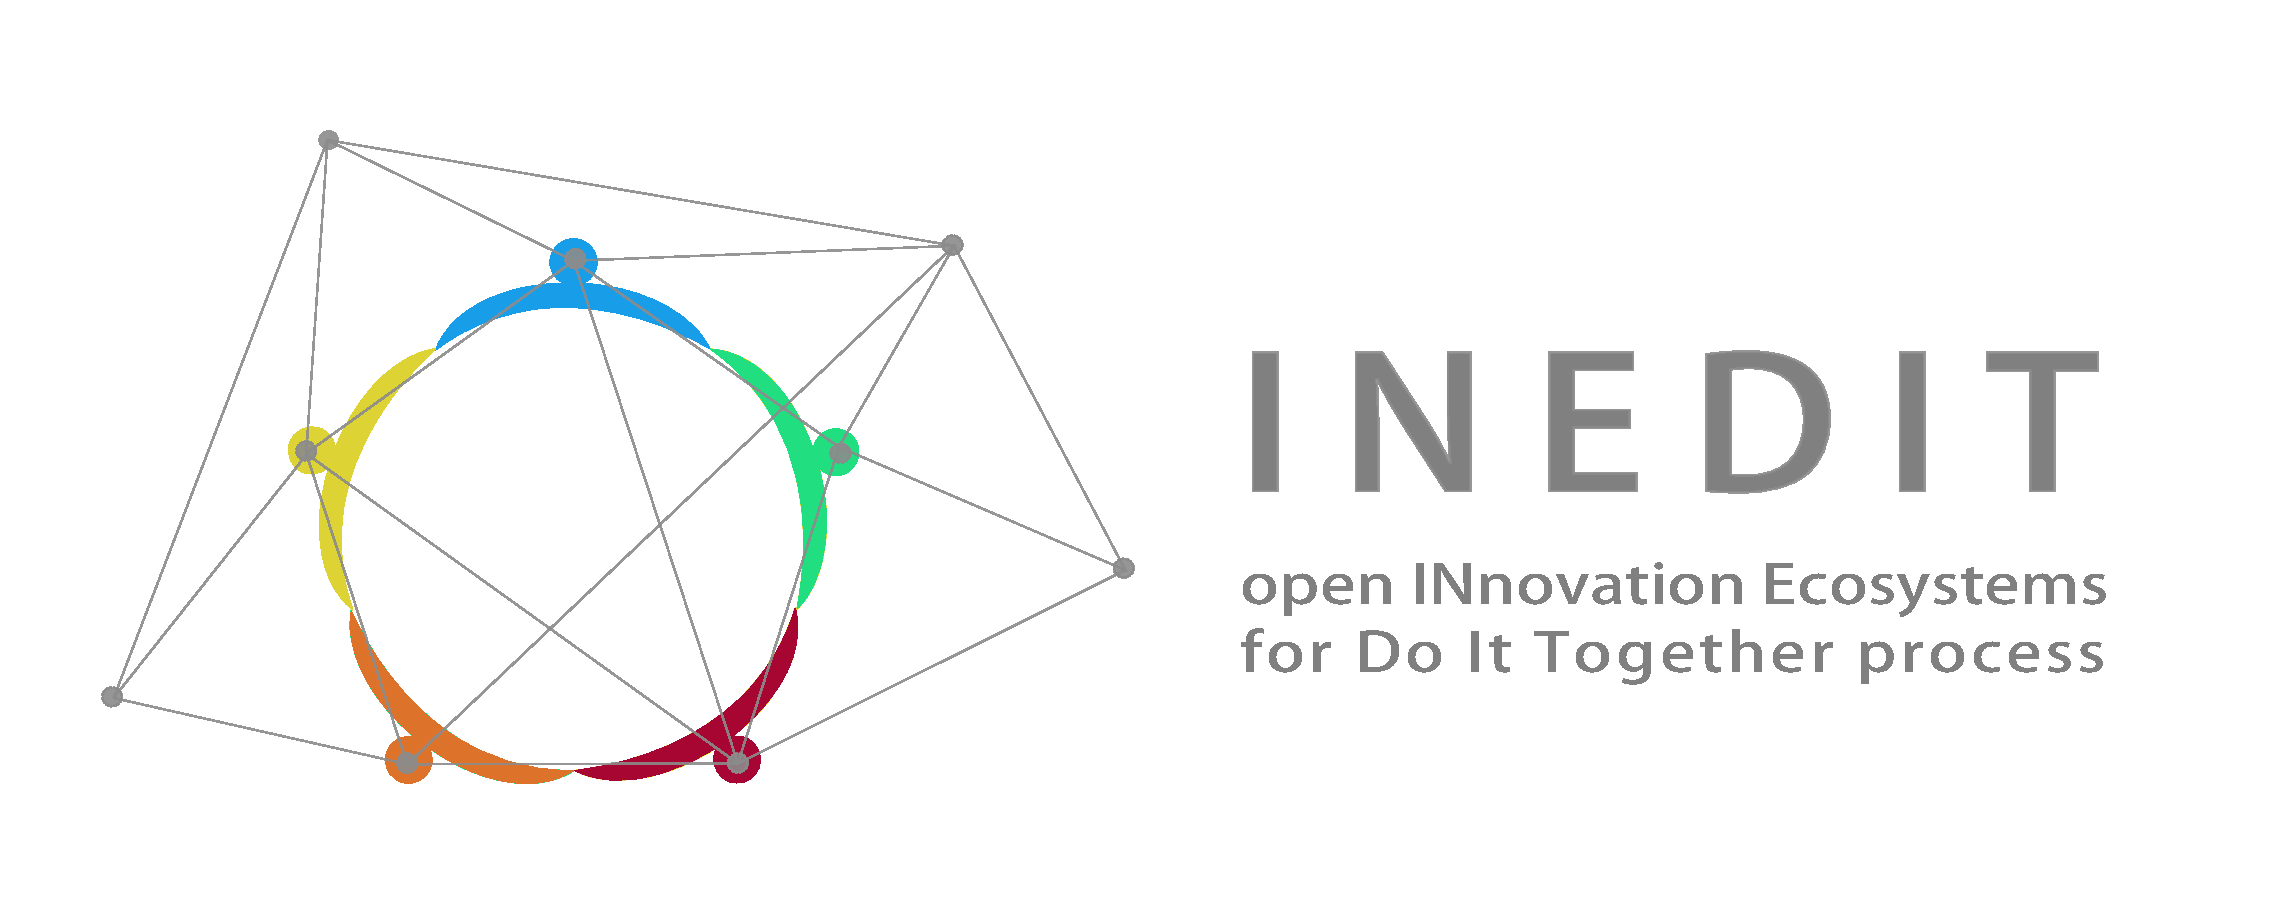
\includegraphics[width=7cm]{figures/Inedit_horiz.pdf} } }  & Work Package: & 6   \\ \cmidrule{3-4}
   & & Type of document:  & Deliverable        \\ \cmidrule{3-4}

   & & Due Delivery Date:    & January 31/2023     \\ \cmidrule{3-4}
 
   & & Actual Delivery Date:    & March 2023       \\ \midrule
 

\multicolumn{4}{l|}{ } \\ \midrule

 Responsible:    &  \multicolumn{3}{|l}{Université de Lorraine }        \\ \midrule
        
 Dissemination Level    &  \multicolumn{3}{|l}{ Public }  \\ \midrule
 Title:    &   \multicolumn{3}{|l}{ Report on the 3D printing of Recycled Plastic Demonstrator }    \\ \hline

 Description:    &    \multicolumn{3}{| p{\dimexpr0.75\linewidth-2\tabcolsep\relax}}{
Description of the conceptual framework of distributed recycling via additive manufacturing (DRAM) and its concrete implementation in a DIT approach. The technologies, materials and methods are reported. Several illustrative case studies are presented.
}   \\ \midrule
 
 
 \multicolumn{1}{l|}{Version}     &   \multicolumn{3}{|l}{ Version 3}    \\ \midrule
 \multicolumn{1}{l|}{Contributors}       & Versions    & Dates       & Revision Description \\ \midrule
\multicolumn{1}{l|}{WP6 Leader} & 0 & February 04/2023 & Validation of the global structure  \\ \midrule        
\multicolumn{1}{l|}{UL} & 1 & March 03/2022 & Revision of a version 1 \\ \midrule
\multicolumn{1}{l|}{UL and SCM} & 2 & March 17/2022 & Revision of a version 2 given the received comments \\ \midrule        
\end{tabu}


\vfill

\begin{center}
\textcolor{lightgray}{Disclaimer}

\textcolor{lightgray}{
\small
This document is provided « as is » with no warranties whatsoever, including any warranty or merchantability, non-infringement, fitness for any particular purpose, or any warranty otherwise arising out of any proposal, specification or sample.  No license, express or implied, by estoppels or otherwise, to any intellectual property rights are granted herein. The members of the project INEDIT do not accept any liability for actions or omissions of INEDIT members or third parties and disclaim any obligation to enforce the use of this document. }

\textcolor{lightgray}{
This document reflects only the authors' view and the Commission is not responsible for any use that may be made of the information it contains.  This document is subject to change without notice. 
}
\end{center}
\normalsize


\newpage

\vfill



\textbf{Scientific editor:} \newline
Asst. Prof. Fabio A. CRUZ SANCHEZ, Task Leader – ORCID: \href{https://orcid.org/0000-0001-8529-5327}{https://orcid.org/0000-0001-8529-5327} \newline
Université de Lorraine, ERPI, F-54 000 Nancy, France \newline
Contact: fabio.cruz@univ-lorraine.fr 

\vspace{2cm}

\textbf{Authors:} \newline
PhD. Fabio A. CRUZ SANCHEZ, M.Sc. Cristian CACERES-MENDOZA, PhD. Fedoua KASMI, PhD. Laurent DUPONT \newline
Université de Lorraine, ERPI, F-54000 Nancy, France \newline
Contact: fabio.cruz@univ-lorraine.fr 

\vspace{2cm}

\textbf{Acknowledgment:}\newline
The authors express their gratitude to the INEDIT consortium. 
Additionally, appreciation is extended to the 'Octroi Nancy' Local Third Place and the local actors in Nancy who actively participated in the experimentation of the smart collector. 
Lastly, the authors acknowledge the valuable scientific collaboration with the Western University in Ontario, Canada, 
Universidade de Vigo in Spain, 
and  LRGP (Université de Lorraine) and CESI School in France.
\vspace{2cm}

\textbf{How to cite:} \newline
Fabio A. Cruz Sanchez, Cristian Caceres Mendoza, Fédoua Kasmi, Laurent Dupont. 
INEDIT Project - Deliverable 6.4 - 3D Printing of recycled plastic demonstrator. 
Université de Lorraine; European Union’s Horizon 2020 research and innovation programme. 2023 ⟨hal-04371315⟩


\vfill
\newpage
